% !TEX root = ../thesis.tex
% \chapter{Results and discussion}
\chapter{Surface-surface interaction based separation of magnetic particles}
\section{Characterization of superparamagnetic particles}
\subsection{Zeta potential}

\subsection{Magnetophoretic velocity}
To ensure the \acp{MP} of different chemical functionalization have the same magnetic content and differences in the mean velocity are solely based on the electrostatic interactions, the magnetophoretic velocity far away from any wall has been measured.
This ensures that no surface-surface interaction occurs, and the velocity measured is based on the magnetic content.
To do so, a large fluid chamber was 3D printed where the \ac{MP} solution was placed of $\qtyproduct{11 x 11 x 2}{\milli\meter}$ with a bar magnet attached to one wall, which can be seen in \textbf{Figure \ref{fig:mag_phor_velocity_with_mag_field}} (b).

\begin{figure}
    \centering
    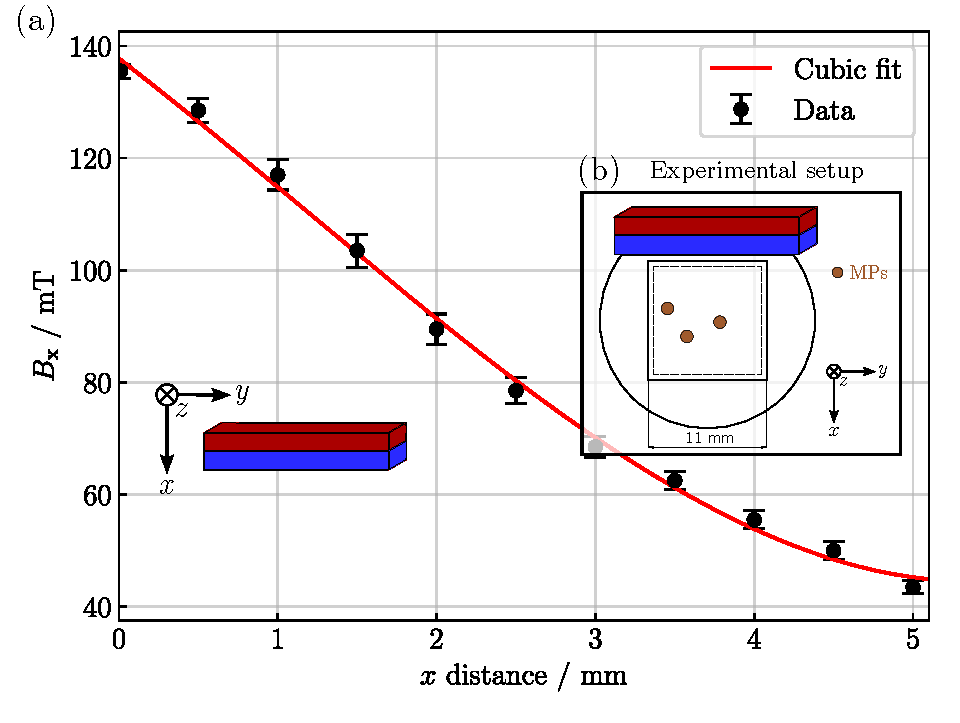
\includegraphics[width=0.8\linewidth]{Abbildungen/Experimental/vMagPho.pdf}
    \caption{
            (a) Magnetic flux density in the investigated magnet orientation for different distances from the neodymium magnet attached to the wall at $x=0$.
            (b) Top view of the experimental setup using a neodymium magnet with a 3D-printed fluid chamber sealed by a coverslip (not shown).
            Taken from \cite{Shubbak2026}  in the Supplemental Material.
            }
    \label{fig:mag_phor_velocity_with_mag_field}
\end{figure}

To further ensure no wall interaction, the focal plane of the microscope was set to be in the center of the container. 
The magnetic gradient field attracts the \acp{MP} towards $x=0$, and this movement was captured with the camera. 
$B_\mathrm{x}(x)$ in dependence of the distance to the magnet can be seen in Figure \ref{fig:mag_phor_velocity_with_mag_field} (a).
The resulting mean magnetophoretic velocity $\left< \left< u \right> \right>$ was used to calculate the magnetic susceptibility $\chi_\mathrm{MP}$ using\cite{Wise2015}
\begin{equation}
    \left< \left< u \right> \right> = \frac{V(\chi_\mathrm{MP}-\chi_\mathrm{fl})}{6\pi r \eta}\frac{\left| \nabla B^2\right|}{2\mu_0},
\end{equation}
with the magnetic flux density $B_\mathrm{x}(x)$ of the bar magnet.
Videos with durations between \SI{10}{\s} and \SI{50}{\s} were recorded through the dark-field microscope with a 20$\,\times\,$ magnification objective. 
A total of 442 trajectories for \ch{COOH} and 155 trajectories for \ch{NH2} functionalized \acp{MP} of the micromod micromer®-M were evaluated as the \acp{MP} used in the mean velocity study of different surface functionalization.
At a distance of \SI{2}{mm} away from the magnet surface, i.e., at \SI{88.0}{\mT}, $\left< \left< u_\mathrm{COOH} \right> \right> = \SI{149\pm16}{\micro\m\per\s}$ and $\left< \left< u_\mathrm{NH2} \right> \right> = \SI{151\pm14}{\micro\m\per\s}$ were found. 
The resulting $\chi_\mathrm{MP}$ are $\chi_\mathrm{\ch{COOH}} = 0.26\pm0.01$ and $\chi_\mathrm{\ch{NH2}} = 0.26\pm0.01$, which is comparable to literature\cite{Grob2018}.

\section{Transport dynamics close to the surface}
\subsection{Mean ensemble velocity}\label{subsection:mean_velocity}
In this Section, the mean velocity $\left< v \right>$ of the particle ensemble transported close to the substrate's surface will be the main focus. 
It will be presented how the mean velocity is calculated considering a constant video duration, but with a varying number of steps each particle can take, or with a constant number of steps but, therefore, a varying video duration.
It will be shown that keeping the number of steps constant has benefits while granting a reasonably high statistic.
The used \acp{MP} are the micromer®-M particles from micromod with $r=\SI{1}{\micro\m}$ and either a carboxygroup or a mixture of a carboxygroup and an aminegroup at their respective surfaces.   

\subsubsection{Ratchet-like transport}
Using pulsed field traveling wave magnetophoresis (see Paragraph \ref{para:PFTWM}) with a distinct trapizoidal field shape, the magnetic potential energy landscape transformation creates a transport that is observable as a ratchet jumping motion.
Due to the transport mechanism, four distinct parts are present:
First, a positive field in $x$ gives an initial tilt above a \ac{DW} along the transport direction.
This initial transformation of the energy landscape pushes the \ac{MP} for a short distance, usually less than  \SI{2}{\micro\m}, appearing as a small step.
Then, the applied $z$ field changes polarity, and the superposition of the magnetic fields creates new minima at the adjacent \ac{DW}.
Accordingly, an energy maximum is now present at the \ac{DW} where the \ac{MP} was residing, which pushes the particle physically higher.
Since the landscape is slightly skewed in the direction of transport by the applied $x$ field, the \ac{MP} does not randomly fall onto one or the other adjacent potential minima, but it has a preferred direction along $x$.
This is now observable as a large step which, in sum with the small step, will cover $\nicefrac{1}{2}d$, that is, the distance from one \ac{DW} to the next.
In an $x$ over $t$ graph, the two steps are separated by a stationary phase. 
Such a graph is presented in Figure \ref{fig:x-t-graph} for the linear regime.

\begin{figure}
    \centering
    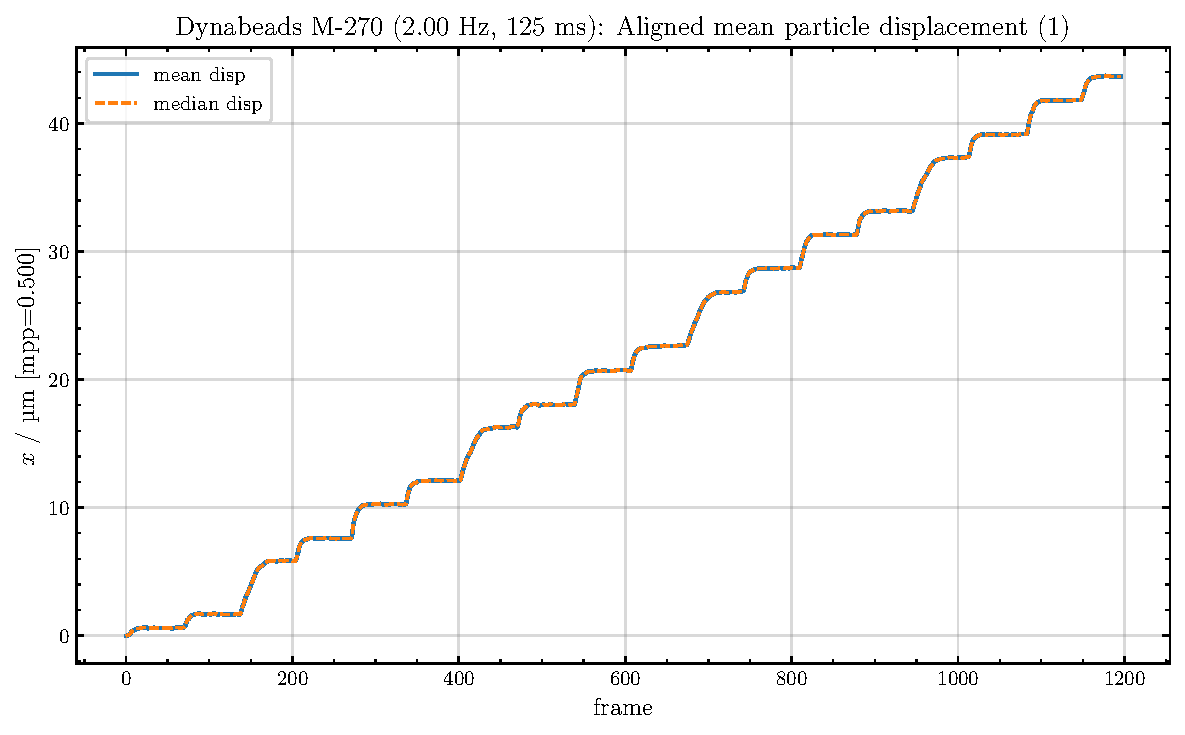
\includegraphics[width=1\linewidth]{Abbildungen/Evaluation/xvst_mean_Dynabeads M-270 (2.00 Hz, 125 ms).pdf}
    \caption{PLATZHALTER WEIL KOMISCHE DATEN
    $x$ over $t$ graph of a transport experiment in the linear regime.
    }
    \label{fig:x-t-graph}
\end{figure}


\section{Transport of magnetic particles bound to proteins}
A major step towards a useful \ac{LOC} system is to prove that \acp{MP} can, indeed, be distinguished in their transport properties once bound to molecules. 
The following chapter will answer the question of how to efficiently transport proteins bound to particles and, consequently, how to detect that binding.
A mean velocity analysis similar to the one shown in Section \ref{subsection:mean_velocity} will be presented further, cementing the feasibility of the transport and detection concept.
The influence of different protein concentrations will be discussed, comparing Zeta potentials and the mean ensemble transport velocities.


\subsection{Sample preparation}

\subsection{Physiological conditions for proteins}


\subsection{Influence on Zeta potential?}
\subsection{Transport dynamics?}

\chapter{Particle transport on tissue}
\section{Sample preparation}
\section{Transport dynamics}

\subsection{Steady-state velocity?}

\chapter{White light interferometer for absolute height determination?}




